\documentclass[11pt]{article}
\usepackage[margin=1in]{geometry}
\usepackage{fontspec}
\usepackage{booktabs}
\usepackage{array}
\usepackage{float}
\usepackage{graphicx}
\usepackage{adjustbox}
\usepackage{amsmath}
\usepackage[font=small,labelfont=bf]{caption}
\usepackage{natbib}
\usepackage{xurl}
\usepackage[hidelinks]{hyperref}
\usepackage{setspace}
\setstretch{1.15}
\graphicspath{{../figs/}}
\newcommand{\nTotal}{2,222}
\newcommand{\nDem}{1,024}
\newcommand{\nRep}{1,198}
\newcommand{\shownRich}{4}
\newcommand{\anesRich}{4.6}
\newcommand{\shownAtheist}{14}
\newcommand{\anesAtheistStrict}{12.6}
\newcommand{\guessRich}{30}
\newcommand{\overRich}{96}
\newcommand{\guessOld}{40}
\newcommand{\overOld}{85}
\newcommand{\overAtheist}{69}
\newcommand{\overNonwhite}{44}
\newcommand{\repTellAsk}{0.043}
\newcommand{\repTellAskCI}{[0.017, 0.069]}
\newcommand{\repTellAskP}{0.001}
\newcommand{\repTellAskHolm}{0.02}
\newcommand{\repAskControl}{-0.020}
\newcommand{\repAskControlP}{0.11}
\newcommand{\repTellControl}{0.023}
\newcommand{\repTellControlP}{0.08}
\newcommand{\repControlMean}{0.47}
\newcommand{\demTellAsk}{-0.003}
\newcommand{\demTellAskCI}{[-0.031, 0.025]}
\newcommand{\gapTellAsk}{0.046}
\newcommand{\gapTellAskP}{0.02}
\newcommand{\minExpressiveHolm}{0.41}
\newcommand{\minInPartyP}{0.13}
\newcommand{\weightedRepTellAsk}{0.044}
\newcommand{\weightedRepTellAskP}{0.03}
\newcommand{\minUndercoverP}{0.22}
\newcommand{\demErrorSD}{14}
\newcommand{\demErrorInteraction}{-0.036}
\newcommand{\demErrorInteractionP}{0.01}
\newcommand{\demErrorInteractionHolm}{0.10}
\newcommand{\repStereoInteractionP}{0.70}
\newcommand{\moreLikeDem}{21}
\newcommand{\moreLikeRep}{38}
\newcommand{\moreLikeDebriefRep}{36}

\newcommand{\TableStyle}{\small\setlength{\tabcolsep}{5pt}\renewcommand{\arraystretch}{1.05}}

\title{The Social Construction of Partisanship: Misperceptions about Party Composition and Partisan Identification}
\author{Douglas J. Ahler \and Gaurav Sood}
\date{}

\begin{document}
\maketitle

\begin{abstract}
\noindent A leading account holds that people identify with the party whose members look like them. Americans overestimate how many of a party's supporters belong to party-stereotypical groups, so correcting those beliefs tells most partisans that their party is more like them than they thought. We ran the correction as an experiment on \nTotal{} weak and leaning partisans in a probability panel. Republicans told the true shares of evangelicals, seniors, and the rich in their party felt more attached to it than Republicans who only guessed, by \repTellAsk{} on a 0--1 scale. Democrats told the true shares of atheists, young people, and nonwhites did not move. Neither party's members changed their party identification, and the effect among Republicans was no larger for those who had overestimated more or who belonged to fewer of the stereotyped groups. The results contradict the claim that group concerns bind Democrats more than Republicans, and they give no support to the matching mechanism the group account proposes.
\end{abstract}

\section{Introduction}

Why do Americans who know little about policy hold on to their parties so tightly? One answer is that party identification is a group attachment: people picture the kinds of people who make up each party and join the party whose picture includes them \citep{green2002, campbell1960, achen2016}. A recent synthesis splits the difference by party, arguing that Democrats are a coalition of groups while Republicans are bound by ideology \citep{grossmann2016}. Both claims rest on circumstantial evidence, such as stable party ties through policy shifts and the predictive power of group membership after controlling for policy views.

We test the group account directly. People overestimate the share of a party's supporters who belong to groups stereotypically linked to it, such as the rich among Republicans and atheists among Democrats \citep{ahler2018}. Most partisans do not belong to these groups, so learning the true, smaller shares tells them that their party looks more like them than they thought. If people identify with the party that looks like them, the correction should strengthen identification, and it should do so most for people who overestimated most and for people outside the stereotyped groups.

The correction raised Republicans' attachment to their party and left Democrats' unchanged, the reverse of the asymmetry the synthesis predicts. Neither the size of the misperception nor the respondent's own group memberships moderated the effect. Party identification on the standard seven-point scale did not move in either party.

\section{Design}

Time-sharing Experiments for the Social Sciences (TESS) funded the experiment, and NORC fielded it on AmeriSpeak, a probability panel of US adults, from April 10 to 29, 2018. The sample was \nTotal{} panelists who had previously placed themselves at 2, 3, 5, or 6 on the seven-point party identification scale: weak partisans and leaners, \nDem{} Democrats and \nRep{} Republicans. We excluded strong partisans and pure independents because their attachments have little room to move. Within each of the four party-identification categories, respondents were assigned with equal probability to one of three arms:

\begin{description}
\item[Ask] Respondents guessed what percentage of their party's supporters belonged to three groups, then answered the outcome questions.
\item[Tell] Respondents guessed, saw the true share for each group and how far off they were, said whether the party was more, as much, or less like them than they had thought, and then answered the outcome questions.
\item[Control] Respondents answered the outcome questions first and guessed at the end.
\end{description}

Democrats were asked about atheists or agnostics, adults aged 18 to 34, and nonwhites; Republicans about evangelical Christians, adults 65 and older, and people earning \$250,000 or more a year. The true shares come from the 2016 American National Election Study, counting leaners as partisans (Table~\ref{tab:guesses}). Two of the shares we showed differ slightly from what a strict reading of the ANES gives. We told Republicans that \shownRich\% earn \$250,000 or more; the ANES figure is \anesRich\%. We told Democrats that \shownAtheist\% are atheist or agnostic, a figure that also counts people who call themselves secular; atheists and agnostics alone are \anesAtheistStrict\%.

The two outcomes are an expressive partisanship index and seven-point party identification. The index averages four items about the respondent's pre-survey party, each scored from 0 to 1: how much it upsets the respondent when people criticize the party, how connected they feel when they meet its supporters, how often they say ``we'' rather than ``they'' about them, and how they feel when the party does well in polls \citep{huddy2015}. Party identification uses the standard branching questions, oriented so that 7 means a strong identifier with the pre-survey party and 1 a strong identifier with the other party. Every respondent stood at 5 or 6 before the survey.

The Tell vs.\ Ask comparison isolates the information, because both arms guessed before the outcomes. Ask vs.\ Control isolates the effect of being asked to guess, and Tell vs.\ Control combines the two. All estimates are differences in means conditional on the four randomization blocks, with HC2 standard errors. We report all three comparisons for both outcomes and both parties. Holm-adjusted $p$-values correct for the 18 tests across parties, the pooled sample, and outcomes. The pre-survey covariates are balanced across arms (Table~\ref{tab:balance}).

\section{Results}

Partisans overestimated the stereotyped groups, Republicans especially (Table~\ref{tab:guesses}). The median Republican guessed that \guessRich\% of Republicans earn \$250,000 or more, and \overRich\% of Republicans guessed above the true share. The median guess for Republicans 65 and older was \guessOld\%, and \overOld\% overestimated. Democrats' errors were smaller and mixed: \overAtheist\% overestimated the share of atheists and agnostics, but only \overNonwhite\% overestimated the share of nonwhites.

\begin{table}[H]
\centering
\caption{Shares shown in the tell arm, ANES 2016 shares, and respondents' guesses}
\label{tab:guesses}
{\TableStyle\adjustbox{max width=\linewidth}{
\begin{tabular}{lrrrrrr}
\toprule
Group & Shown & ANES 2016 & Median guess & Mean guess & Share overestimating & n\\
\midrule
\addlinespace[0.3em]
\multicolumn{7}{l}{\textit{Democrats asked about Democrats}}\\
\hspace{1em}Atheist or agnostic & 14 & 14.2 & 20 & 26.5 & 69 & 635\\
\hspace{1em}Age 18-34 & 30 & 30.4 & 36 & 39.1 & 57 & 648\\
\hspace{1em}Nonwhite & 43 & 42.6 & 40 & 41.4 & 44 & 640\\
\addlinespace[0.3em]
\multicolumn{7}{l}{\textit{Republicans asked about Republicans}}\\
\hspace{1em}Evangelical & 37 & 37.1 & 40 & 41.5 & 56 & 772\\
\hspace{1em}Age 65+ & 21 & 21.3 & 40 & 43.3 & 85 & 769\\
\hspace{1em}Earn \$250,000+ & 4 & 4.6 & 30 & 33.5 & 96 & 774\\
\bottomrule
\end{tabular}
}}
\par\smallskip
\begin{minipage}{0.95\linewidth}\footnotesize
Note: Shares are percentages of the respondent's own party. ANES 2016 shares are weighted and count leaners as partisans. Guesses are from the ask and tell arms, made before the outcome questions. Share overestimating is the percentage of respondents whose guess exceeded the share shown.
\end{minipage}
\end{table}

The correction strengthened Republicans' attachment to their party (Figure~\ref{fig:effects}, Table~\ref{tab:effects}). Republicans who saw the true shares scored \repTellAsk{} higher on the expressive index than Republicans who only guessed (95\% CI \repTellAskCI{}, $p = \repTellAskP$, Holm-adjusted $p = \repTellAskHolm$). Against a control mean of \repControlMean{}, the effect is modest. The Democratic estimate is \demTellAsk{} (\demTellAskCI{}), and the difference between the parties is \gapTellAsk{} ($p = \gapTellAskP$). Weighting to the population gives a Republican estimate of \weightedRepTellAsk{} ($p = \weightedRepTellAskP$; Table~\ref{tab:robustness}).

Part of the Republican Tell vs.\ Ask contrast comes from the ask arm. Guessing alone lowered Republicans' attachment by \repAskControl{} relative to control ($p = \repAskControlP$), and the tell arm sits \repTellControl{} above control ($p = \repTellControlP$). One possibility is that Republicans who wrote down large shares of the rich and the old came away thinking less of their party; the design cannot test it. No other comparison on the expressive index survives the Holm adjustment (smallest adjusted $p = \minExpressiveHolm$).

\begin{figure}[H]
\centering
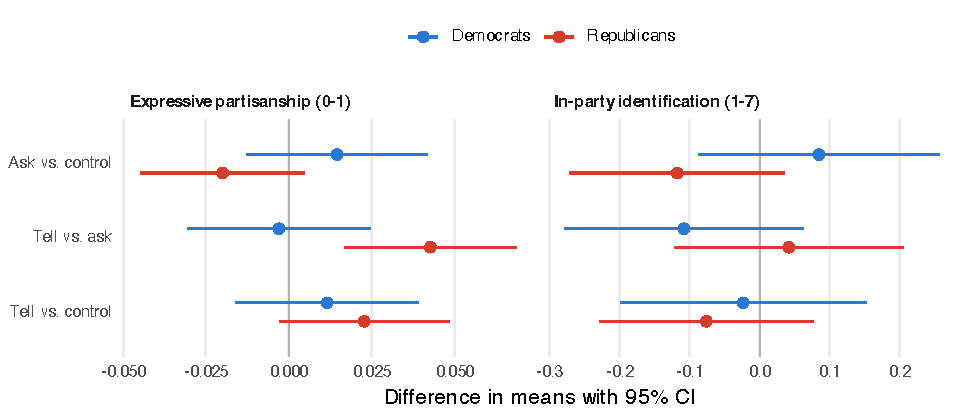
\includegraphics[width=\linewidth]{effects.pdf}
\caption{Effects of guessing and of correction on attachment to the pre-survey party. Points are differences in means conditional on randomization blocks; bars are 95\% confidence intervals from HC2 standard errors. Expressive partisanship runs from 0 to 1; in-party identification is the seven-point scale oriented toward the pre-survey party.}
\label{fig:effects}
\end{figure}

\begin{table}[H]
\centering
\caption{Effects on attachment to the pre-survey party}
\label{tab:effects}
{\TableStyle\adjustbox{max width=\linewidth}{
\begin{tabular}{lrrrr}
\toprule
Contrast & Democrats & Republicans & Pooled & Rep. - Dem.\\
\midrule
\addlinespace[0.3em]
\multicolumn{5}{l}{\textit{Expressive partisanship (0-1)}}\\
\hspace{1em}Ask vs. control & 0.015 (0.014) & -0.020 (0.013) & -0.004 (0.009) & -0.034* (0.019)\\
\hspace{1em}Tell vs. ask & -0.003 (0.014) & 0.043*** (0.013) & 0.022** (0.010) & 0.046** (0.019)\\
\hspace{1em}Tell vs. control & 0.012 (0.014) & 0.023* (0.013) & 0.018* (0.010) & 0.011 (0.019)\\
\addlinespace[0.3em]
\multicolumn{5}{l}{\textit{In-party identification (1-7)}}\\
\hspace{1em}Ask vs. control & 0.085 (0.088) & -0.118 (0.078) & -0.024 (0.058) & -0.202* (0.117)\\
\hspace{1em}Tell vs. ask & -0.108 (0.087) & 0.042 (0.083) & -0.027 (0.060) & 0.150 (0.120)\\
\hspace{1em}Tell vs. control & -0.024 (0.089) & -0.076 (0.078) & -0.051 (0.059) & -0.053 (0.119)\\
\bottomrule
\end{tabular}
}}
\par\smallskip
\begin{minipage}{0.95\linewidth}\footnotesize
Note: Differences in means conditional on randomization blocks, with HC2 standard errors in parentheses. The last column is the Republican minus the Democratic effect from a model with arm-by-party interactions. Stars mark unadjusted $p<0.1$, $0.05$, $0.01$; the text reports Holm-adjusted $p$-values.
\end{minipage}
\end{table}

Attachment moved, but identification did not. No comparison on the seven-point scale reaches conventional significance in either party (smallest $p = \minInPartyP$). Among leaners, the correction did not change how many called themselves independent rather than Democrat or Republican (smallest $p = \minUndercoverP$; Table~\ref{tab:robustness}), so it did not draw out the ``undercover'' partisans \citet{klar2016} describe.

The group account also predicts who should respond: people who overestimated most, since they learn the most, and people outside the stereotyped groups, since they learn the party is like them. Neither prediction holds among Republicans (Table~\ref{tab:moderation}). Their effect is flat across the size of the misperception and across the number of stereotyped groups they belong to ($p = \repStereoInteractionP$). Among Democrats, those who overestimated more grew slightly \emph{less} attached when corrected: \demErrorInteraction{} per standard deviation of guess error (\demErrorSD{} points; $p = \demErrorInteractionP$, Holm-adjusted $p = \demErrorInteractionHolm$). This sign is the opposite of the group account's prediction.

\begin{table}[H]
\centering
\caption{Moderation of the information effect (tell vs.\ ask)}
\label{tab:moderation}
{\TableStyle\adjustbox{max width=\linewidth}{
\begin{tabular}{llrrrr}
\toprule
Party & Moderator & Tell vs. ask at mean & Tell x moderator (per SD) & Holm p & n\\
\midrule
\addlinespace[0.3em]
\multicolumn{6}{l}{\textit{Expressive partisanship (0-1)}}\\
\hspace{1em}Democrats & Mean guess error & -0.014 (0.014) & -0.036** (0.014) & 0.10 & 627\\
\hspace{1em}Republicans & Mean guess error & 0.040*** (0.013) & 0.006 (0.013) & 1.00 & 765\\
\hspace{1em}Democrats & Share of stereotyped groups & -0.003 (0.014) & 0.020 (0.014) & 1.00 & 669\\
\hspace{1em}Republicans & Share of stereotyped groups & 0.043*** (0.013) & 0.005 (0.013) & 1.00 & 792\\
\addlinespace[0.3em]
\multicolumn{6}{l}{\textit{In-party identification (1-7)}}\\
\hspace{1em}Democrats & Mean guess error & -0.130 (0.090) & -0.026 (0.083) & 1.00 & 626\\
\hspace{1em}Republicans & Mean guess error & 0.002 (0.083) & -0.020 (0.090) & 1.00 & 765\\
\hspace{1em}Democrats & Share of stereotyped groups & -0.108 (0.087) & 0.038 (0.091) & 1.00 & 668\\
\hspace{1em}Republicans & Share of stereotyped groups & 0.048 (0.081) & -0.007 (0.080) & 1.00 & 792\\
\bottomrule
\end{tabular}
}}
\par\smallskip
\begin{minipage}{0.95\linewidth}\footnotesize
Note: Each row is one regression on the ask and tell arms of the treatment, the centered moderator, their product, and randomization blocks, with HC2 standard errors. Mean guess error is the respondent's guess minus the share shown, averaged over the three groups, in percentage points. Share of stereotyped groups is the fraction of the three groups the respondent belongs to; the panel's top income bracket, \$200,000 or more, stands in for \$250,000. Interactions are per standard deviation of the moderator. Holm adjustment is over the eight interactions. Guesses in the control arm came after the outcomes, so moderation uses only the ask and tell arms.
\end{minipage}
\end{table}

The manipulation check fits this pattern. On the correction screen, \moreLikeRep\% of Republicans and \moreLikeDem\% of Democrats said their party was more like them than they had thought (Table~\ref{tab:reactions}). Republicans in the ask and control arms, who saw the same correction at the end of the survey, answered much the same (\moreLikeDebriefRep\%).

\section{Discussion}

Learning that their party is less stereotypical than they believed made Republicans feel closer to it and left Democrats unmoved. If the synthesis were right that Democrats are the party of group interests and Republicans the party of ideology \citep{grossmann2016}, the result should have run the other way. The correction also failed to move party identification itself, and it worked no better for the respondents the group account says it should reach. If partisans judged their party by how much it looked like them, those respondents should have moved most.

Two features of the design limit what the null results say. The sample held weak partisans and leaners, so the results describe people whose ties could move, not strong partisans. And the correction concerned three groups per party; a party's image is built from many more. The Republican result suggests that who belongs to a party matters to how its supporters feel about it. These data do not support the group account's explanation, that it matters through the match between the respondent and the party.

\bibliographystyle{apsr}
\bibliography{references}

\appendix
\section*{Appendix}
\setcounter{table}{0}
\renewcommand{\thetable}{A\arabic{table}}

\begin{table}[H]
\centering
\caption{Covariate balance by arm}
\label{tab:balance}
{\TableStyle\adjustbox{max width=\linewidth}{
\begin{tabular}{lrrrr}
\toprule
Covariate & Control & Ask & Tell & Joint p\\
\midrule
\addlinespace[0.3em]
\multicolumn{5}{l}{\textit{Democrats}}\\
\hspace{1em}Age & 45.64 & 45.85 & 45.66 & 0.97\\
\hspace{1em}Female & 0.48 & 0.47 & 0.47 & 0.97\\
\hspace{1em}White, non-Hispanic & 0.53 & 0.51 & 0.55 & 0.54\\
\hspace{1em}Bachelor's degree & 0.25 & 0.25 & 0.28 & 0.62\\
\hspace{1em}Ideology (1-7, conservative high) & 3.44 & 3.45 & 3.40 & 0.88\\
\hspace{1em}Income (1-18) & 9.08 & 9.06 & 9.11 & 0.98\\
\hspace{1em}Leaner & 0.47 & 0.50 & 0.47 & 0.36\\
\hspace{1em}Share of stereotyped groups & 0.30 & 0.31 & 0.31 & 0.84\\
\addlinespace[0.3em]
\multicolumn{5}{l}{\textit{Republicans}}\\
\hspace{1em}Age & 49.07 & 48.69 & 49.10 & 0.96\\
\hspace{1em}Female & 0.50 & 0.51 & 0.53 & 0.82\\
\hspace{1em}White, non-Hispanic & 0.83 & 0.78 & 0.81 & 0.39\\
\hspace{1em}Bachelor's degree & 0.43 & 0.42 & 0.41 & 0.72\\
\hspace{1em}Ideology (1-7, conservative high) & 5.02 & 4.96 & 5.00 & 0.86\\
\hspace{1em}Income (1-18) & 10.77 & 10.37 & 10.36 & 0.28\\
\hspace{1em}Leaner & 0.51 & 0.55 & 0.51 & 0.18\\
\hspace{1em}Share of stereotyped groups & 0.19 & 0.19 & 0.19 & 0.86\\
\bottomrule
\end{tabular}
}}
\par\smallskip
\begin{minipage}{0.95\linewidth}\footnotesize
Note: Means by arm. Joint $p$ is the robust Wald test that the two arm coefficients are zero in a regression of the covariate on arm and randomization blocks.
\end{minipage}
\end{table}

\begin{table}[H]
\centering
\caption{Weighted estimates and the leaners' party label}
\label{tab:robustness}
{\TableStyle\adjustbox{max width=\linewidth}{
\begin{tabular}{lrrr}
\toprule
Contrast & Democrats & Republicans & Pooled\\
\midrule
\addlinespace[0.3em]
\multicolumn{4}{l}{\textit{Weighted: expressive partisanship}}\\
\hspace{1em}Ask vs. control & 0.015 (0.019) & -0.010 (0.017) & 0.004 (0.013)\\
\hspace{1em}Tell vs. ask & 0.007 (0.020) & 0.044** (0.021) & 0.023 (0.015)\\
\hspace{1em}Tell vs. control & 0.022 (0.019) & 0.034 (0.021) & 0.027** (0.014)\\
\addlinespace[0.3em]
\multicolumn{4}{l}{\textit{Weighted: in-party identification}}\\
\hspace{1em}Ask vs. control & 0.122 (0.138) & -0.028 (0.105) & 0.059 (0.091)\\
\hspace{1em}Tell vs. ask & -0.156 (0.134) & 0.025 (0.118) & -0.078 (0.092)\\
\hspace{1em}Tell vs. control & -0.034 (0.139) & -0.003 (0.103) & -0.019 (0.091)\\
\addlinespace[0.3em]
\multicolumn{4}{l}{\textit{Leaners only: calls self independent}}\\
\hspace{1em}Ask vs. control & -0.009 (0.051) & -0.005 (0.041) & -0.007 (0.032)\\
\hspace{1em}Tell vs. ask & 0.061 (0.050) & -0.019 (0.042) & 0.015 (0.032)\\
\hspace{1em}Tell vs. control & 0.052 (0.050) & -0.024 (0.042) & 0.009 (0.032)\\
\bottomrule
\end{tabular}
}}
\par\smallskip
\begin{minipage}{0.95\linewidth}\footnotesize
Note: Weighted rows use NORC's post-stratification weight, controlled within party. Leaner rows estimate the effect on the share of leaners who answer ``independent'' or ``other'' to the first party identification question. HC2 standard errors in parentheses.
\end{minipage}
\end{table}

\begin{table}[H]
\centering
\caption{Reactions to the correction (percent)}
\label{tab:reactions}
{\TableStyle\adjustbox{max width=\linewidth}{
\begin{tabular}{lrrrr}
\toprule
Reaction & Democrats (tell) & Republicans (tell) & Democrats (ask, control) & Republicans (ask, control)\\
\midrule
More like me & 21 & 38 & 21 & 36\\
As much like me & 38 & 31 & 43 & 36\\
Less like me & 41 & 31 & 37 & 28\\
\bottomrule
\end{tabular}
}}
\par\smallskip
\begin{minipage}{0.95\linewidth}\footnotesize
Note: ``Which statement best captures your reaction to this information? The [party] is more like me / as much like me / less like me than I had thought.'' Tell respondents answered on the correction screen, before the outcomes; ask and control respondents saw the same correction at the end of the survey.
\end{minipage}
\end{table}

\end{document}
